\documentclass[12pt]{beamer}
\usetheme{CambridgeUS}
\usepackage[utf8]{inputenc}
\usepackage[spanish]{babel}
\usepackage{amsmath}
\usepackage{multirow, array}
\usepackage{amsfonts}
\usepackage{amssymb}
\usepackage{graphicx}
\usepackage{ragged2e}
\setbeamertemplate{navigation symbols}{} 
\author[Kevin - Alejandro x2]{Kevin García 1533173 \newline Alejandro Vargas 1525953 \newline Alejandro Soto 1532457}
\title[Diseños factoriales fraccionados]{Diseños factoriales fraccionados}

%\setbeamercovered{transparent} 
%\setbeamertemplate{navigation symbols}{} 
%\logo{} 
%\institute{} 
%\date{} 
%\subject{} 
\begin{document}
\justifying
\begin{frame}[plain]
\maketitle
\end{frame}


\begin{frame}
\frametitle{Introducción}
Los diseños factoriales surgen ante la necesidad de estudiar conjuntamente varios factores obedeciendo a la posibilidad de que el efecto de un factor cambie según los niveles de otros factores, esto es, que los factores interactúen. Estos diseños también se usan cuando se quiere
optimizar la respuesta o variable dependiente, es decir, se quiere encontrar la combinación de niveles de los factores que producen un valor óptimo de la variable dependiente.
~\\Si se investiga un factor por separado, el resultado puede ser diferente al estudio conjunto y es mucho más difícil describir el comportamiento general del proceso o encontrar el óptimo.
\end{frame}

\begin{frame}
\frametitle{Diseño Factorial}
~\\Un diseño factorial es un tipo de experimento cuyo diseño permite estudiar los efectos que varios factores pueden tener en una respuesta. Al realizar un experimento, variar los niveles de todos los factores al mismo tiempo en lugar de uno a la vez, permite estudiar las interacciones entre los factores.

\end{frame}

\begin{frame}
\frametitle{Diseño Factorial}
~\\Suponga que tenemos dos factores, $A$ con a niveles y $B$ con b niveles. Las observaciones de un experimento factorial pueden describirse con un modelo. Hay varias formas de escribir el modelo de un experimento factorial. La forma más utilizada es el modelo de los efectos:
\begin{center}
$y_{ijk}=\mu+\tau_i+\beta_j+(\tau\beta)_{ij}+\varepsilon_{ijk} \;\;\; \left \{\begin{array}{c} i=1,2,...,a \\ j=1,2,...,b \\ k=1,2,...,n \end{array}\right. $
\end{center}
\end{frame}


\begin{frame}
\frametitle{Diseño Factorial}

~\\Donde $\mu$ es el efecto promedio global, $\tau_i$ es el efecto del nivel i-ésimo del factor $A$ de los renglones, $\beta_j$ es el efecto del nivel j-ésimo del factor $B$ de las columnas, $(\tau\beta)_{ij}$ es el efecto de la interacción entre $\tau_i$ y $\beta_j$, y $\varepsilon_{ijk}$ es un componente del error aleatorio. Puesto que hay n replicas del experimento, hay $abn$ observaciones en total.

\end{frame}

\begin{frame}
\frametitle{Diseño Factorial}
~\\El efecto de un factor se define como el cambio en la respuesta producido por un cambio en el nivel del factor, a este efecto se le conoce como efecto principal porque se refiere a los factores de interés primario en el experimento. Entonces si tenemos dos factores A y B, como en la siguiente tabla:
~\\
% Table generated by Excel2LaTeX from sheet 'Hoja1'
\begin{table}[htbp]
  \centering
  \caption{}
    \begin{tabular}{|c|c|c|}
\cline{2-3}    \multicolumn{1}{c|}{} & \multicolumn{2}{c|}{\textbf{Factor A}} \\
    \hline
    \textbf{Factor B} & \textbf{bajo } & \textbf{alto} \\
    \hline
    \textbf{bajo} & a     & b  \\
    \hline
    \textbf{alto} & c     & d  \\
    \hline
    \end{tabular}%
  \label{tab:addlabel}%
\end{table}%
\end{frame}

\begin{frame}
\frametitle{Diseño Factorial}
~\\El efecto principal del factor A es la diferencia entre la respuesta promedio con el nivel alto de A y la respuesta promedio con el nivel bajo de A. Esto es:
$$A=\frac{b+d}{2}-\frac{a+c}{2}$$
~\\Análogamente, el efecto principal del factor B es:
$$B=\frac{c+d}{2}-\frac{a+b}{2}$$  
\end{frame}

\begin{frame}
\frametitle{Diseño Factorial}
~\\Si existe interacción entre los factores A y B, el efecto de la interacción se define como la diferencia promedio de los dos efectos del factor A, es decir:
$$AB=\frac{(d-c)-(b-a)}{2}$$
~\\En el diseño factorial de dos factores, ambos factores, $A$ y $B$ son de igual interés, por lo que se prueban las hipótesis acerca de la igualdad de los efectos de los tratamientos de cada factor. Para el factor $A$:
\begin{center}
~\\$H_0:\tau_1=\tau_2=\cdots=\tau_a=0$
~\\$H_1:$Al menos una $\tau_i\neq 0$
\end{center}
\end{frame}

\begin{frame}
\frametitle{Diseño Factorial}
~\\Para el factor $B$:
\begin{center}
~\\$H_0:\beta_1=\beta_2=\cdots=\beta_b=0$
~\\$H_1:$Al menos una $\beta_j\neq 0$
\end{center}
~\\También existe interés en determinar si los tratamientos de los factores $A$ y $B$ interactúan. Por lo tanto, también querría probarse
\begin{center}
~\\$H_0:(\tau\beta)_{ij}=0$ para todas las $i,j$
~\\$H_1:$Al menos una $(\tau\beta)_{ij}\neq 0$
\end{center}
\end{frame}

\begin{frame}
\frametitle{Diseño Factorial}
~\\Todas las hipótesis anteriores se pueden probar realizando el análisis de varianza de dos factores como sigue:

\begin{table}[htbp]
  \centering
  \caption{ANOVA}
\resizebox{12cm}{!} {
\begin{tabular}{|c|c|c|c|c|}
\hline 
Fuente de Variación & Grados de Libertad & Suma de Cuadrados & Cuadrados Medios & F \\ 
\hline 
$A$ & a-1 & $SC_A$ & $CM_A=\frac{SC_A}{a-1}$ & $F=\frac{CM_{A}}{CM_{error}}$ \\ 
$B$ & b-1 & $SC_B$ & $CM_B=\frac{SC_B}{b-1}$ & $F=\frac{CM_{B}}{CM_{error}}$ \\
$AB$ &(a-1)(b-1) & $SC_{AB}$ & $CM_{AB}=\frac{SC_{AB}}{(a-1)(b-1)}$ & $F=\frac{CM_{AB}}{CM_{error}}$ \\
Error & ab(n-1) & $SC_{error}$ & $CM_{error}=\frac{SC_{error}}{ab(n-1)}$ &   \\ 
Total & abn-1 & $SC_{total}$ &  &   \\ 
\hline 
\end{tabular} 
}
\label{tab:addlabel}%
\end{table}%
\end{frame}

\begin{frame}
\frametitle{Diseño Factorial}
~\\Donde la suma de cuadrados total es:
$$SC_{total}=\sum\limits_{i=1}^a \sum\limits_{j=1}^b \sum\limits_{k=1}^n y^2_{ijk}-\frac{y^2_{\ldots}}{abn}$$

~\\La suma de cuadrados de los efectos principales son:
\begin{center}
$SC_A=\frac{1}{bn}\sum\limits_{i=1}^a y^2_{i..} - \frac{y^2_{\ldots}}{abn}\;\;$ y $\;\;SC_B=\frac{1}{an}\sum\limits_{j=1}^b y^2_{.j.} - \frac{y^2_{\ldots}}{abn}$
\end{center}

\end{frame}

\begin{frame}
\frametitle{Diseño Factorial}
~\\La suma de cuadrados de la interacción es:
$$SC_{AB}=\frac{1}{n}\sum\limits_{i=1}^a\sum\limits_{j=1}^b y^2_{ij.}-\frac{y^2_{\ldots}}{abn}-SC_{A}-SC_{B}$$

~\\Y, la suma de cuadrados del error se encuentra como:
$$SC_{error}=SC_{total}-\frac{1}{n}\sum\limits_{i=1}^a\sum\limits_{j=1}^b y^2_{ij.}-\frac{y^2_{\ldots}}{abn}$$
\end{frame}

\begin{frame}
\frametitle{Ejemplo de Diseño factorial}

\end{frame}

\begin{frame}
\frametitle{Diseño Factorial $2^{k}$}
~\\Existen varios casos especiales del diseño factorial general, los cuales son muy importantes debido a su uso generalizado en el trabajo de investigación. El más importante de estos casos especiales es el diseño de k factores, donde cada factor cuenta con sólo dos niveles. Estos niveles pueden ser tanto cuantitativos como cualitativos. Una réplica completa de este diseño requiere $2 x 2 x\cdots x 2 =2^k$ observaciones y se le llama diseño factorial $2^k$.
\end{frame}

\begin{frame}
\frametitle{Diseño Factorial $ 2^{k} $}
~\\El diseño $2^k$ es de particular utilidad en las etapas iniciales del trabajo experimental, cuando probablemente se estén investigando muchos factores. Este diseño proporciona el menor número de corridas con las que pueden estudiarse k factores en un diseño factorial completo.

~\\El diseño $2^k$ es de particular utilidad en las etapas iniciales del trabajo experimental, cuando probablemente se estén investigando muchos factores. Este diseño proporciona el menor número de corridas con las que pueden estudiarse k factores en un diseño factorial completo.
\end{frame}

\begin{frame}
\frametitle{Diseño Factorial $ 2^{k} $}
~\\El modelo estadístico para un diseño $2^k$ incluiría k efectos principales, $\binom{k}{2}$ interacciones de dos factores, $\binom{k}{3}$ interacciones de tres factores,..., y una interacción de k factores. Es decir, para un diseño $2^k$ el modelo completo contendría $2^k-1$ efectos.

~\\El enfoque general para el análisis estadístico del diseño $2^k$ se resume en la siguiente tabla
\begin{table}[htbp]
  \centering
  \caption{Enfoque del diseño  $ 2^{k} $}
  \resizebox{4.7cm}{!} {
\begin{tabular}{l}
\hline 
1. Estimar los efectos de los factores\\
2. Formar el modelo inicial\\
3. Realizar las pruebas estadísticas\\
4. Refinar el modelo\\
5. Analizar los residuales\\
6. Interpretar los resultados\\
\hline 
\end{tabular}
}
\label{tab:addlabel}%
\end{table}%
\end{frame}

\begin{frame}
\frametitle{Diseño Factorial $ 2^{k} $}
~\\En este diseño, la tabla estándar se construye empezando con el primer factor con el signo(-) y alterna signos (-) y (+). El segundo factor cambia de signo cada dos observaciones ($2^1$), el tercer factor cada cuatro ($2^2$) y el factor k-ésimo cada $2^{k-1}$ observaciones. las interacciones de los factores tienen los signos que se obtienen de multiplicar los signos de los factores implicados. Por ejemplo, en el diseño $2^3$ la tabla estándar con las interacciones es:
\end{frame}

\begin{frame}
\frametitle{Diseño Factorial $ 2^{k} $}
\begin{table}[H]
  \centering
  \caption{Matriz de Diseño}
  \resizebox{0.5\textwidth}{!}{
    \begin{tabular}{cccccccc}
    \hline
    \textbf{A} & \textbf{B} & \textbf{C} & \textbf{AB} & \textbf{AC} & \textbf{BC} & \textbf{ABC} & \textbf{Respuesta y} \\
    \hline
    -     & -     & -     & +     & +     & +     & -     & $y_{111}=(1)$ \\
    +     & -     & -     & -     & -     & +     & +     & $y_{211}=a$ \\
    -     & +     & -     & -     & +     & -     & +     & $y_{121}=b$ \\
    +     & +     & -     & +     & -     & -     & -     & $y_{221}=ab$ \\
    -     & -     & +     & +     & -     & -     & +     & $y_{112}=c$ \\
    +     & -     & +     & -     & +     & -     & -     & $y_{212}=ac$ \\
    -     & +     & +     & -     & -     & +     & -     & $y_{122}=bc$ \\
    +     & +     & +     & +     & +     & +     & +     & $y_{222}=abc$ \\
    \hline
    \end{tabular}%
    }
  \label{tab:addlabel}%
\end{table}%
\end{frame}

\begin{frame}
\frametitle{Diseño Factorial $ 2^{k} $}
~\\En la tabla se logra apreciar que el nivel alto de cualquiera de los factores en una combinación de tratamientos se denota por la letra minúscula correspondiente y que el nivel bajo de un factor en una combinación de tratamientos se denota por la ausencia de la letra respectiva. Por lo tanto, para un diseño $2^2$ a representa la combinación de tratamientos con A en el nivel alto y B en el nivel bajo, b representa A en el nivel bajo y B en el nivel alto, y ab representa ambos factores en el nivel alto. Por convención, se usa (1) para denotar que ambos factores están en el nivel bajo. Esta notación se utiliza en todos los diseños $2^k$.
\end{frame}

\begin{frame}
\frametitle{Diseño Factorial $ 2^{k} $}
~\\Ahora, teniendo en cuenta la notación anterior y que n es el número de réplicas hechas con la combinación de los tratamientos.Para estimar un efecto o calcular la suma de cuadrados de un efecto, primero debe determinarse el contraste asociado con ese efecto. En general, el contraste del efecto $AB\cdots K$ se determina expandiendo el miembro derecho de
$$Contraste_{AB\cdots K}=(a\pm 1)(b\pm 1)\cdots(k\pm 1)$$
~\\Una vez se han calculado los contrastes de los efectos, pueden estimarse los efectos y calcular las sumas de cuadrados de acuerdo con
$$AB\cdots K=\frac{2}{n2^k}(Contraste_{AB\cdots K})$$
~\\y
$$SS_{AB\cdots K}=\frac{1}{n2^k}(Contraste_{AB\cdots K})^2$$

\end{frame}

\begin{frame}
\frametitle{Diseño Factorial $ 2^{k} $}
~\\Entonces el análisis de varianza de un diseño $2^k$ es
\begin{table}[H]
  \centering
  \caption{}
  \resizebox{0.58\textwidth}{!}{
    \begin{tabular}{ccc}
    \hline
    \textbf{Fuente de variación} & \textbf{Suma de cuadrados} & \textbf{Grados de libertad} \\
    \hline
   A & $SS_A$ & 1 \\
   B & $SS_B$ & 1 \\
   \vdots & \vdots & \vdots \\
   K & $SS_K$ & 1 \\
   AB & $SS_{AB}$ & 1 \\
   AC & $SS_{AC}$ & 1 \\
   \vdots & \vdots & \vdots \\
   JK & $SS_{JK}$ & 1 \\
   ABC & $SS_{ABC}$ & 1\\
   ABD & $SS_{ABD}$ & 1\\
   \vdots & \vdots & \vdots\\
   IJK & $SS_{IJK}$ & 1\\
   \vdots & \vdots & \vdots \\
   $ABC\cdots K$ & $SS_{ABC\cdots K}$ & 1\\
   Error & $SS_{E}$ & $2^k(n-1)$ \\
   Total & $SS_{T}$ & $n2^k-1$ \\
    \hline
    \end{tabular}%
    }
  \label{tab:addlabel}%
\end{table}%
\end{frame}

\begin{frame}
\frametitle{Diseños Factoriales Fraccionados}
~\\En un diseño factorial conforme el número de factores del experimento crece, el número de casillas o condiciones experimentales (y por lo tanto el número de lecturas o pruebas necesarias), crece exponencialmente, también crece el número de efectos a evaluar (interacciones principalmente) y el número de efectos y casillas varía con el número de factores en una relación como se muestra en la tabla siguiente para un experimento factorial $2^k$.
\end{frame}

\begin{frame}
\frametitle{Diseño Factorial Fraccionado}
% Table generated by Excel2LaTeX from sheet 'Hoja1'
\begin{table}[htbp]
  \centering
  \caption{No de factores del experimento}
  \resizebox{0.7\textwidth}{!}{
    \begin{tabular}{|c|c|c|c|c|c|c|c|c|c|}
    \hline
    \multicolumn{1}{|c|}{\multirow{2}[4]{*}{\textbf{No. De \newline{} factores}}} & \multicolumn{1}{c|}{\multirow{2}[4]{*}{\textbf{No. De \newline{} casillas}}} & \multicolumn{1}{c|}{\multirow{2}[4]{*}{\textbf{Efectos \newline{} principales}}} & \multicolumn{7}{c|}{\textbf{Interacciones entre factores }} \\
\cline{4-10}          &       &       & 2     & 3     & 4     & 5     & 6     & 7     & 8 \\
    \hline
    2     & 4     & 2     & 1     &       &       &       &       &       &  \\
    \hline
    3     & 8     & 3     & 3     & 1     &       &       &       &       &  \\
    \hline
    4     & 16    & 4     & 6     & 4     & 1     &       &       &       &  \\
    \hline
    5     & 32    & 5     & 10    & 10    & 5     & 1     &       &       &  \\
    \hline
    6     & 64    & 6     & 15    & 20    & 15    & 6     & 1     &       &  \\
    \hline
    7     & 128   & 7     & 21    & 35    & 35    & 27    & 7     & 1     &  \\
    \hline
    8     & 256   & 8     & 28    & 58    & 70    & 56    & 28    & 8     & 1 \\
    \hline
    \end{tabular}%
    }
  \label{tab:addlabel}%
\end{table}%
En general el número de interacciones de k factores tomados r en r es:

$$kCr=\frac{k!}{r!(k-r)!}$$
\end{frame}

\begin{frame}
\frametitle{Diseño Factorial Fraccionado}
~\\El concepto de replicación fraccionada se  basa en 3 hipótesis:

\begin{enumerate}[1.]
    \item Las interacciones de tres o más factores son sumamente raras en la práctica, por lo que en general se pueden suponer como no existentes.
    \item En un experimento de varios factores lo más probable es que solo algunos de ellos sean relevantes para la variable de respuesta.
    \item La mayor parte del efecto se debe a los factores principales y algunas interacciones de dos factores.
\end{enumerate}
\end{frame}

\begin{frame}
~\\Cuando solamente una parte de las posibles casillas se prueban, se dice que se tiene una replicación fraccionada del experimento.

~\\Las preguntas que surgen son:

\begin{enumerate}[1.]
    \item ¿Cuántas y cuales casillas probar?
    \item ¿Cómo analizar los resultados?
    \item ¿Qué información se pierde?
\end{enumerate}

~\\El objetivo del diseño factorial fraccionado (replicación fraccionada) es darle respuesta a estos interrogantes.

\end{frame}

\begin{frame}
\frametitle{Fracción un medio de un diseño $ 2^{k} $}
~\\Ahora nos enfocaremos en este tipo de diseño, donde se utiliza la mitad de las corridas del diseño completo $2^k$, ya que este es el diseño más importante y más utilizado en la práctica.

~\\Para explicar más fácil este método nos centraremos en un ejemplo en la que tres factores, cada uno con dos niveles, son de interés. Suponiendo que los experimentadores no están en posición de correr las $2^3=8$ combinaciones de tratamientos, la lógica sugeriría disminuir las corridas. Si se pueden llevar cuatro corridas, esto sugiere una fracción un medio del diseño $2^3$. Puesto que el diseño contiene $2^{3-1}=4$ combinaciones de tratamientos, es común llamar diseño $2^{3-1}$ a una fracción un medio del diseño $2^3$.
\end{frame}

\begin{frame}
\frametitle{Fracción un medio de un diseño $ 2^{k} $}
~\\Supongamos que se seleccionan las cuatro combinaciones de tratamientos a,b,c y abc como la fracción un medio con la que se trabajará. En la siguiente tabla se muestra la agrupación de signos positivos y negativos del diseño $2^3$ la cuál se utilizará para explicar el proceso.
% Table generated by Excel2LaTeX from sheet 'Hoja1'
\begin{table}[htbp]
  \centering
  %\caption{Add caption}
  \resizebox{0.65\textwidth}{!}{
    \begin{tabular}{ccccccccc}
    \hline
    \multicolumn{1}{p{7.285em}}{Combinación de } & \multicolumn{8}{c}{Efecto factorial} \\
\cline{2-9}    \multicolumn{1}{p{7.285em}}{tratamientos} & I     & A     & B     & C     & AB    & AC    & BC    & ABC \\
    \hline
    \multicolumn{1}{l}{a} & +     & +     & -     & -     & -     & -     & +     & + \\
    \multicolumn{1}{l}{b} & +     & -     & +     & -     & -     & +     & -     & + \\
    \multicolumn{1}{p{7.285em}}{c } & +     & -     & -     & +     & +     & -     & -     & + \\
    \multicolumn{1}{l}{abc} & +     & +     & +     & +     & +     & +     & +     & + \\
    \hline
    \multicolumn{1}{l}{ab } & +     & +     & +     & -     & +     & -     & -     & - \\
    \multicolumn{1}{l}{ac} & +     & +     & -     & +     & -     & +     & -     & - \\
    \multicolumn{1}{l}{bc} & +     & -     & +     & +     & -     & -     & +     & - \\
    \multicolumn{1}{l}{(1)}    & +     & -     & -     & -     & +     & +     & +     & - \\
    \end{tabular}%
    }
  \label{tab:addlabel}%
\end{table}%
\end{frame}


\begin{frame}
\frametitle{Fracción un medio de un diseño $ 2^{k} $}
~\\Observemos que el diseño $2^{3-1}$ se forma seleccionando sólo las combinaciones de tratamientos que tienen signo positivo en la columna ABC. Por lo tanto, a ABC se le llama generador de esta fracción particular. Además, se observa que la columna identidad I también es totalmente positiva, por lo que a
$$I=ABC$$

~\\se le llama la relación de definición del diseño. En general, la relación de definición de un diseño factorial fraccionado será siempre el conjunto de todas las columnas que son iguales a la columna identidad I. 
\end{frame}

\begin{frame}
\frametitle{Fracción un medio de un diseño $ 2^{k} $}
~\\Se observa que las combinaciones lineales de las observaciones usadas para estimar los efectos principales de A, B y C son
\begin{center}
~\\$l_{A}=\frac{1}{2}(a-b-c+abc)$
~\\$l_{B}=\frac{1}{2}(-a+b-c+abc)$
~\\$l_{C}=\frac{1}{2}(-a-b+c+abc)$
\end{center}
~\\también se observa que las combinaciones lineales de las observaciones usadas para estimar las interacciones de dos factores son:
\begin{center}
~\\$l_{BC}=\frac{1}{2}(a-b-c+abc)$
~\\$l_{AC}=\frac{1}{2}(-a+b-c+abc)$
~\\$l_{AB}=\frac{1}{2}(-a-b+c+abc)$
\end{center}
\end{frame}

\begin{frame}
\frametitle{Fracción un medio de un diseño $ 2^{k} $}
~\\Por lo tanto $l_{A}=l_{BC}$,$l_{B}=l_{AC}$ y $l_{C}=l_{AB}$; por consiguiente, es imposible diferenciar entre A y BC, entre B y AC y entre C y AB. De hecho, cuando se estiman A, B y C, se están estimando en realidad $A+BC$, $B+AC$ y $C+AB$. A dos o más efectos que tienen esta propiedad se les llama alias. En este ejemplo, A y BC son alias, al igual que B y AC y C y AB.
\end{frame}

\begin{frame}
\frametitle{Coeficiente Lg}
~\\Los coeficientes Lg se pueden observar en la siguiente tabla:
\begin{center}
\resizebox{12cm}{!}{
\begin{tabular}{cccc}
\hline
 &Percepción previa & Percepción posterior &      MFA\\
Percepción previa   &         1.0839432     &       0.7761085 &1.0105158\\
Percepción posterior       &  0.7761085        &    1.0384112 &0.9857795\\
MFA                       &   1.0105158         &   0.9857795 &1.0845333\\
\hline 
\end{tabular}
} 
\end{center}
~\\El valor del coeficiente $Lg_{(P.Previa)}=1.0839$ para la percepción previa indica que es de dimensionalidad uno, es decir, que puede sintetizarse en un solo factor; $Lg_{(P.Posterior)}=1.0384$ indica que la percepción posterior también tiene una dimensión o factor que lo caracteriza. El coeficiente Lg cruzado $Lg_{(P.Prev,P.Post)}=0.7761$ indica que estos dos grupos comparten un factor; y finalmente, el coeficiente $Lg_{(MFA)}=1.0845$ indica que éste se puede sintetizar como mínimo en un factor.
\end{frame}

\begin{frame}
\frametitle{Coeficiente Rv de Escoufier}
~\\ Es una generalización multivariada del coeficiente de correlación de Pearson al cuadrado. Este coeficiente mide el vínculo entre dos grupos o dos matrices de variables. Este coeficiente, al igual que el de correlación de Pearson, se encuentra entre 0(todas las variables del primer grupo o matriz, son ortogonales a todas las variables del segundo grupo o matriz) y 1(los dos grupos o matrices son homotéticos)

~\\El coeficiente de RV se define como (Robert y Escoufier, 1976; Schlich, 1996):

$$RV(W_i,Wj)=\frac{T(W_i,W_j)}{\left[T(W_i,W_i)\cdot T(W_j,W_j)\right]^\frac{1}{2}}$$
\end{frame}

\begin{frame}
\justifying
\frametitle{Coeficiente Rv de Escoufier}
~\\Donde $T(W_i,W_j)=\sum\limits_{l,m}w_{l,m}^i w_{l,m}^j$ es un coeficiente de covarianza generalizado entre las matrices $W_i$ y $W_j$, $T(W_i,W_i)=\sum\limits_{l,m}{w_{l,m}^i}^2 $ es una varianza generalizada de la matriz $W_i$ y $w_{l,m}^2$ es el (l,m) elemento de la matriz $W_i$.

~\\Los coeficientes Rv se pueden observar en la siguiente tabla:
\begin{center}
\resizebox{12cm}{!}{
\begin{tabular}{cccc}
\hline
 &Percepción previa &Percepción posterior   &    MFA \\
Percepción previa &           1.0000000      &      0.7315340& 0.9320054\\
Percepción posterior&         0.7315340       &     1.0000000& 0.9289101\\
MFA                  &        0.9320054        &    0.9289101& 1.0000000\\
\hline 
\end{tabular} 
}
\end{center}
\end{frame}

\begin{frame}
\justifying
\frametitle{Coeficiente Rv de Escoufier}
~\\Los valores de los coeficientes $Rv_{(MFA,P.Previa)}=0.932$ y $Rv_{(MFA,P.Posterior)}=0.9289$ nos indican que ambos grupos (percepción previa y posterior) tienen una estructura cercana a la de toda la degustación ó en otras palabras, tienen un grado considerable de asociación con el AFM. Es decir, que su representación sobre los planos generados por el AFM es adecuada. Además, entre la percepción previa y posterior el coeficiente Rv es de 0.7315340 lo que significa que existe un vinculo considerable entre estos dos grupos (algunas de las variables del primer grupo están asociadas con las del segundo grupo).
\end{frame}

\begin{frame}
\frametitle{Representación superpuesta}
\begin{figure}[h]
  \centering
  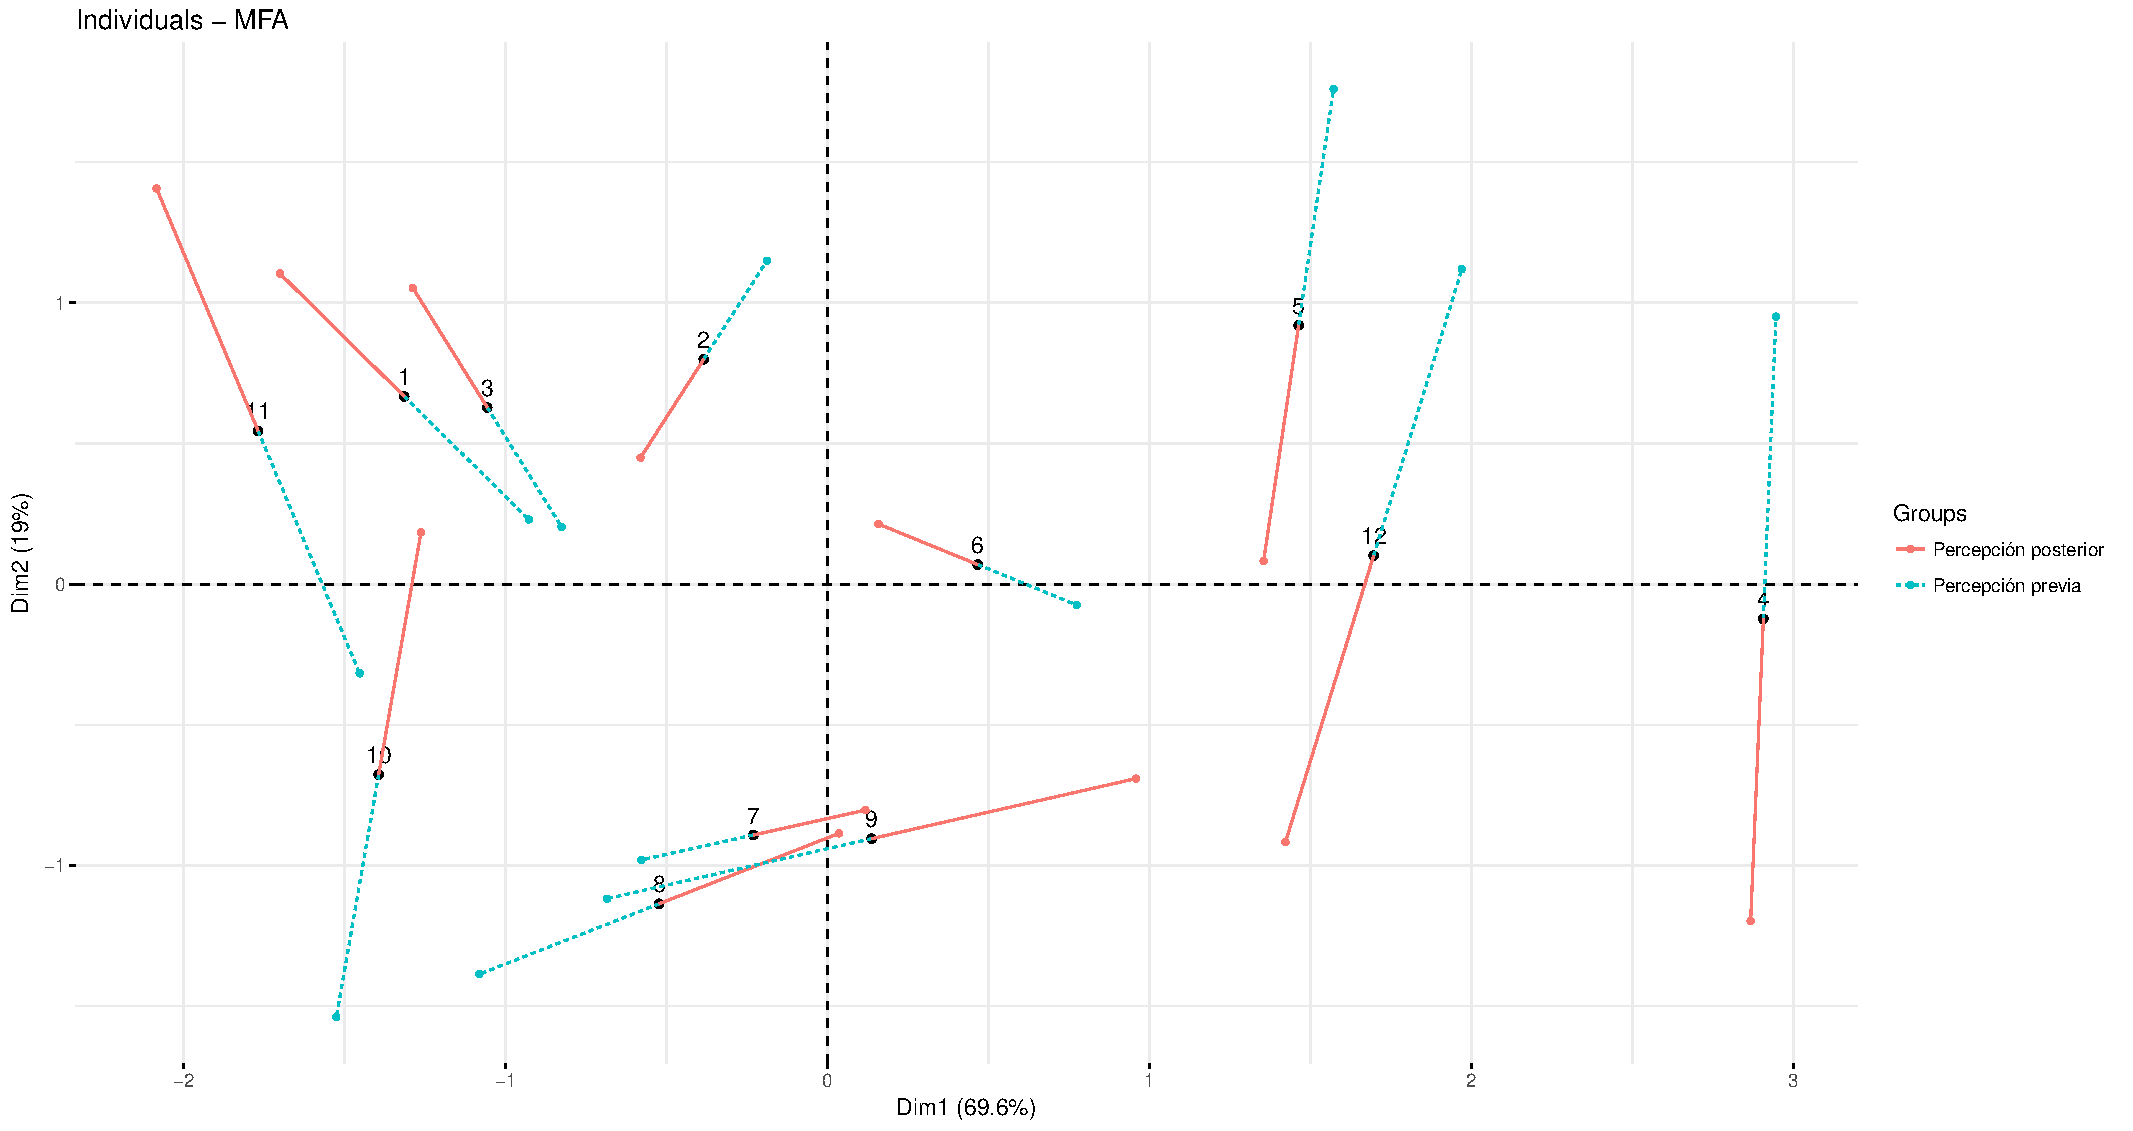
\includegraphics[scale=0.34]{imagenes/RS.pdf}
\end{figure}
\end{frame}

\begin{frame}
\frametitle{Ejes parciales}
\begin{figure}[h]
  \centering
  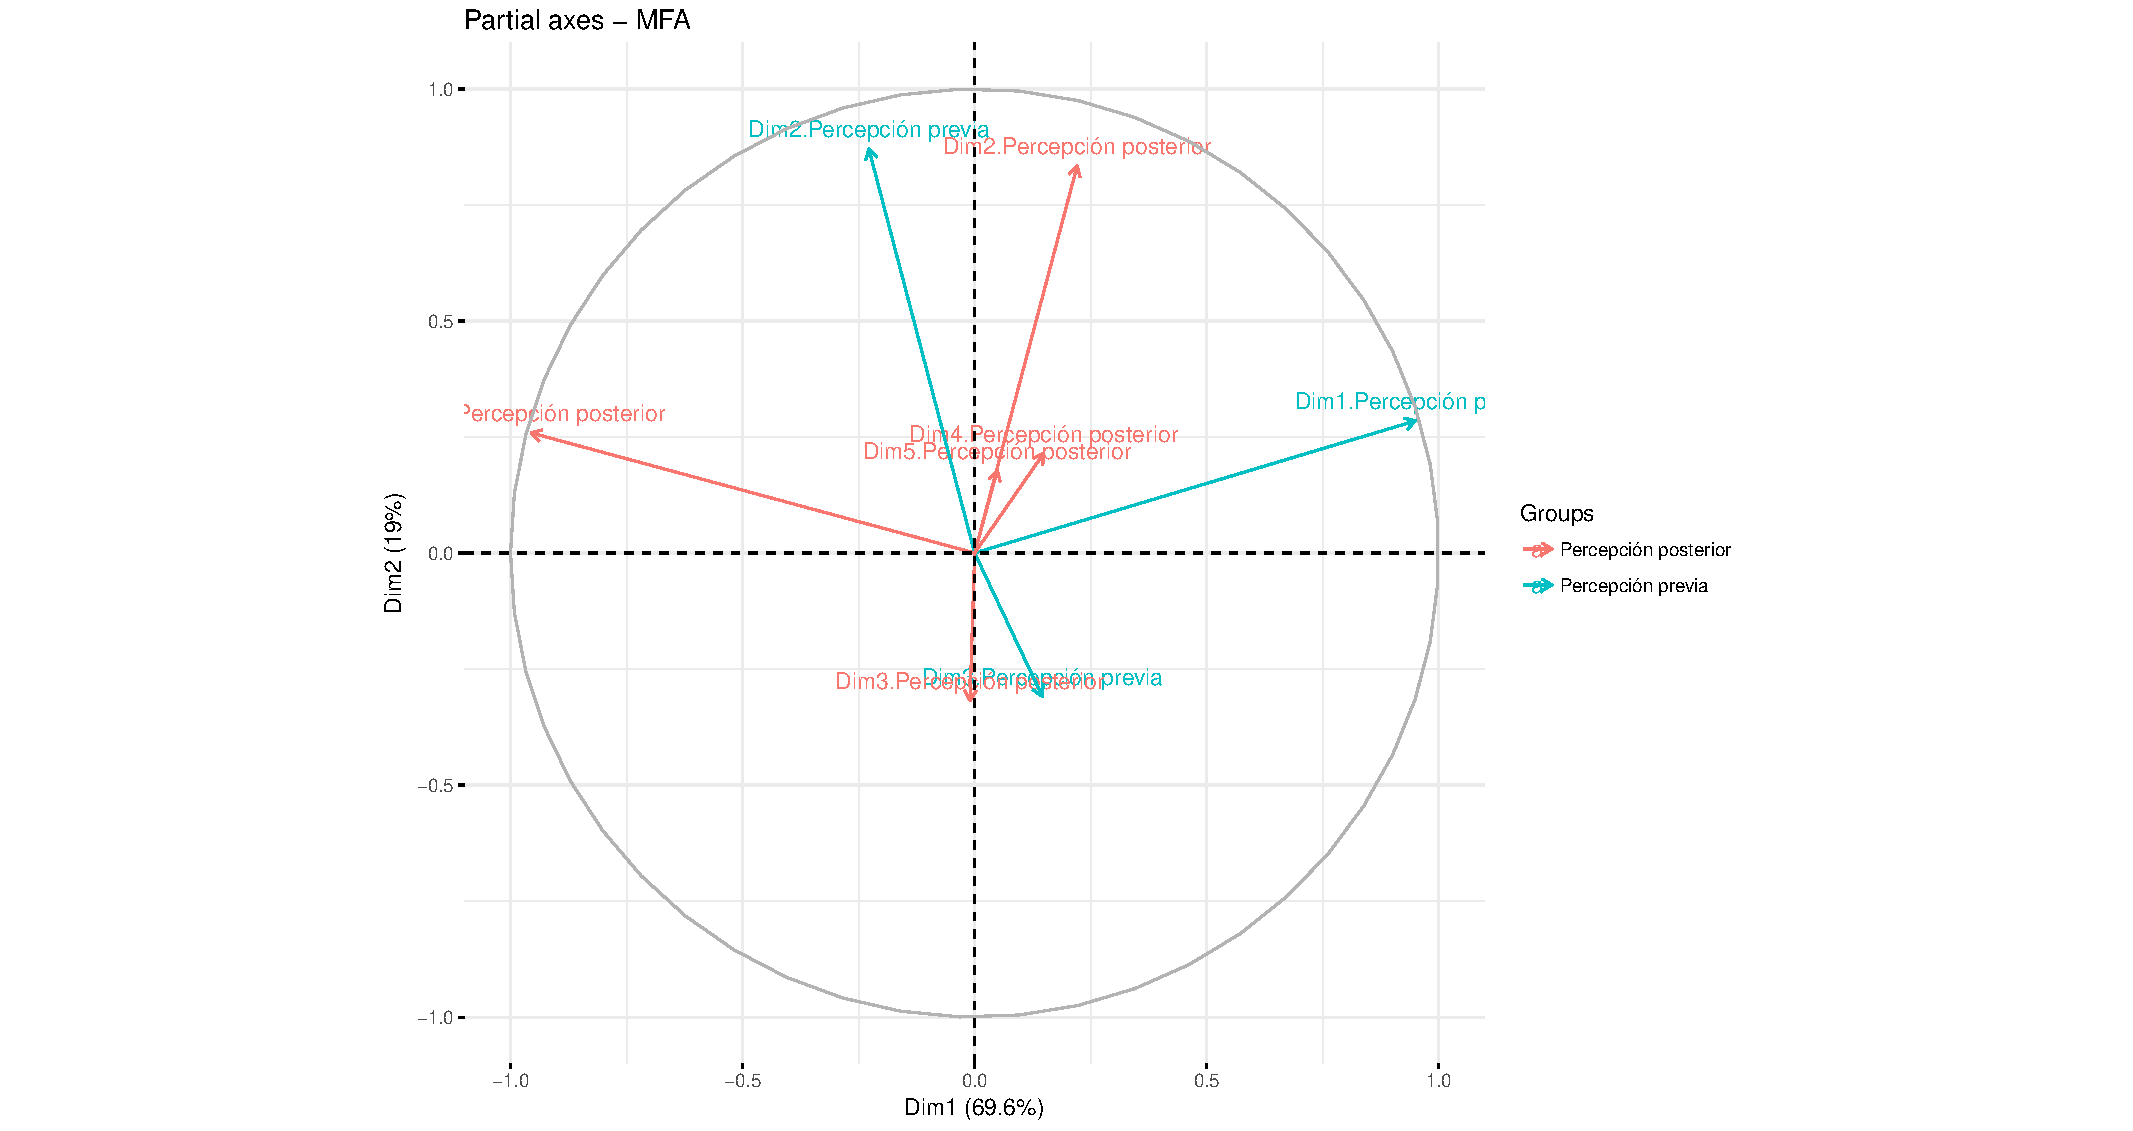
\includegraphics[scale=0.34]{imagenes/EP.pdf}
\end{figure}
\end{frame}

\begin{frame}
\frametitle{Construcción indice}
Las coordenadas de las variables para las dos primeras dimensiones son:

\begin{center}
\resizebox{10cm}{!}{
\begin{tabular}{ccc}
\hline 
 & Dim.1  &    Dim.2   \\   
\hline   
Color.intensity &  0.8581049&  0.2236407 \\ 
Odor.intensity  &  0.6316557&  0.7028833 \\
Attack.intensity & 0.9522195& -0.2260020  \\
Sweet           & -0.8881581& -0.1346408  \\
Acid             & 0.9028145& -0.3139184  \\
Bitter           & 0.9640321&  0.1981328 \\
Pulp             &-0.6320766&  0.7018089 \\
Typicity         &-0.8054955&  0.3978624  \\
\hline
\end{tabular}
}
\end{center}
\end{frame}

\begin{frame}
\frametitle{Construcción indice}
~\\El indice para el primer grupo (percepción previa) es:
$$I=0.8581049 Color+0.6316557 Odor+0.9522195 Attack$$
\begin{center}
\resizebox{3cm}{!}{
\begin{tabular}{cc}
\hline 
 Jugo & Indice  \\   
\hline   
1 & 11.03415 \\
2 &  11.823 \\
3 & 11.16971\\ 
4 & 16.35666\\
5 & 14.28656\\ 
6 & 13.58883\\ 
7 & 11.71434\\ 
8 & 11.12588\\ 
9 & 11.61305\\ 
10& 10.57015\\ 
11& 10.35774\\ 
12& 14.9813 \\  
\hline
\end{tabular}
}
\end{center}
\end{frame}

\begin{frame}
\frametitle{Referencias}
\begin{itemize}
\item Kassambara, A. \& Mundt, F. (2017), factoextra: Extract and Visualize the Results of Multivariate
Data Analyses. R package version 1.0.5.
*https://CRAN.R-project.org/package=factoextra


\item Lê, S., Josse, J. \& Husson, F. (2008), 'FactoMineR: A package for multivariate analysis', Journal
of Statistical Software 25(1), 1-18.


\item Ludovic Lebart, Alain Morineau, M. P. (1995), Statistique exploratoire multidimensionnelle, Dunod,
Paris.

\item Salamanca, J. A. C. (2017), 'Análisis factorial múltiple para clasificación de universidades latinoamericanas', Comunicaciones en Estadística .
\end{itemize}
\end{frame}

\begin{frame}
\frametitle{Referencias}
\begin{itemize}
\item Wickham, H. (2009), ggplot2: Elegant Graphics for Data Analysis, Springer-Verlag New York.
*http://ggplot2.org


\item Wickham, H. \& Bryan, J. (2018), readxl: Read Excel Files. R package version 1.1.0.
*https://CRAN.R-project.org/package=readxl


\item Zelaya, J. T. (n.d.), ANÁLISIS MULTIVARIADO DE DATOS, Universidad de Costa Rica.
\end{itemize}
\end{frame}

\end{document}